\chapter{Population Study of \Acstitle{LAT}-detected \Acsptitle{PWN}}
\chaplabel{population_study}

\paperref{This chapter is based the second part of the the paper
  ``Constraints on the Galactic Population of TeV Pulsar Wind Nebulae using Fermi Large Area Telescope Observations''
  by Acero et al which is currently in prep.}

In \chapref{extended_search}, we search for new spatially-extended \fermi
sources and found that spatial extenion was an important characteristic
for detecting new \acp{PWN}. In the process, we discovered three
new $\gamma$-ray emitting \acp{PWN} candidates
(\hessj{1616}, \hessj{1632}, \hessj{1837}).

In \chapref{offpeak}, we then
searched in the off-peak phase interval of \ac{LAT}-detected pulsars
for new pulsar wind nebula and discovered \threecfiftyeight.  Finally,
in \chapref{tevcat} we searched in the regions surrounding \acp{PWN}
candidates detected at \tev energies for \gev-emitting \acp{PWN}
4 new PWNe candidates (\hessj{1119}, \hessj{1303}, \hessj{1420},
and \hessj{1841}) and 1 new PWN (\hessj{1356})

In this chapter, we take the population of $\gamma$-ray emitting \acp{PWN}
and \acp{PWN} candidates and study how thier multiwavelenth properties
vary with properties of the associated pulsar.


\begin{deluxetable}{ccccccc}

\tabletypesize{\scriptsize}
\tablecolumns{7}
\tablewidth{0pt}
\tablecaption{The muliwavelenth propergies of the \ac{VHE} source and their associated \ac{LAT}-detected pulsar.
\todo[inline]{Add figure caption to this table/make sure it automatically generates figure label}
\tablabel{pwn_multiwavelenth_properties}}

\tablehead{\colhead{Source} & \colhead{$F_{1\unitspace\tev}^{30\unitspace\tev}$} & \colhead{$F_{1\unitspace\kev}^{10\unitspace\kev}$} & \colhead{PSR} & \colhead{$\dot{E}$} & \colhead{$\tau$} & \colhead{Distance}\\ \colhead{ } & \colhead{($10^{-12}\erg\unitspace\cm^{-2}\second^{-1}$)} & \colhead{($10^{-12}\erg\unitspace\cm^{-2}\second^{-1}$)} & \colhead{ } & \colhead{($\erg\unitspace\second^{-1}$)} & \colhead{(kyr)} & \colhead{(kpc)}}
\startdata
VERJ0006+727 & \nodata & \nodata & PSRJ0007+7303 & 4.5e+35 & 13.9 & $1.4 \pm 0.3$ \\
Crab & $80 \pm 16$ & $21000 \pm 4200$ & PSR J0534+2200 & 4.6e+38 & 1.2 & $2.0 \pm 0.5$ \\
MGROJ0631+105 & \nodata & \nodata & PSRJ0631+1036 & 1.7e+35 & 43.6 & $1.00 \pm 0.20$ \\
MGROJ0632+17 & \nodata & \nodata & PSRJ0633+1746 & 3.2e+34 & 342 & $0.2_{-0.1}^{+0.2}$ \\
Vela-X & $79 \pm 21$ & $54 \pm 11$ & PSRJ0835-4510 & 6.9e+36 & 11.3 & $0.29 \pm 0.02$ \\
HESSJ1018-589 & $0.9 \pm 0.4$ & \nodata & PSRJ1016-5857 & 2.6e+36 & 21 & 3 \\
HESSJ1023-575 & $4.8 \pm 1.7$ & \nodata & PSRJ1023-5746 & 1.1e+37 & 4.6 & 2.8 \\
HESSJ1026-582 & $5.9 \pm 4.4$ & \nodata & PSRJ1028-5819 & 8.4e+35 & 90 & $2.3 \pm 0.3$ \\
HESSJ1119-614 & $2.3 \pm 1.2$ & \nodata & PSRJ1119-6127 & 2.3e+36 & 1.6 & $8.4 \pm 0.4$ \\
HESSJ1303-631 & $27 \pm 1$ & $0.16 \pm 0.03$ & PSRJ1301-6305 & 1.7e+36 & 11 & $6.7_{-1.2}^{+1.1}$ \\
HESSJ1356-645 & $6.7 \pm 3.7$ & $0.06 \pm 0.01$ & PSRJ1357-6429 & 3.1e+36 & 7.3 & $2.5_{-0.4}^{+0.5}$ \\
HESSJ1418-609 & $3.4 \pm 1.8$ & $3.1 \pm 0.1$ & PSRJ1418-6058 & 4.9e+36 & 1 & $1.6 \pm 0.7$ \\
HESSJ1420-607 & $15 \pm 3$ & $1.3 \pm 0.3$ & PSRJ1420-6048 & 1.0e+37 & 13 & $5.6 \pm 0.9$ \\
HESSJ1458-608 & $3.9 \pm 2.4$ & \nodata & PSRJ1459-6053 & 9.1e+35 & 64.7 & 4 \\
HESSJ1514-591 & $20 \pm 4$ & $29 \pm 6$ & PSRJ1513-5906 & 1.7e+37 & 1.56 & $4.2 \pm 0.6$ \\
HESSJ1554-550 & $1.6 \pm 0.5$ & $3.1 \pm 1.0$ & \nodata & \nodata & 18 & $7.8 \pm 1.3$ \\
HESSJ1616-508 & $21 \pm 5$ & $4.2 \pm 0.8$ & PSRJ1617-5055 & 1.6e+37 & 8.13 & $6.8 \pm 0.7$ \\
HESSJ1632-478 & $15 \pm 5$ & $0.43 \pm 0.08$ & \nodata & 3.0e+36 & 20 & 3 \\
HESSJ1640-465 & $5.5 \pm 1.2$ & $0.46 \pm 0.09$ & \nodata & 4.0e+36 & \nodata & \nodata \\
HESSJ1646-458B & $5.0 \pm 2.0$ & \nodata & PSRJ1648-4611 & 2.1e+35 & 110 & $5.0 \pm 0.7$ \\
HESSJ1702-420 & $9.0 \pm 3.0$ & $0.01 \pm 0.00$ & PSRJ1702-4128 & 3.4e+35 & 55 & $4.8 \pm 0.6$ \\
HESSJ1708-443 & $23 \pm 7$ & \nodata & PSRJ1709-4429 & 3.4e+36 & 17.5 & $2.3 \pm 0.3$ \\
HESSJ1718-385 & $4.3 \pm 1.6$ & $0.14 \pm 0.03$ & PSRJ1718-3825 & 1.3e+36 & 89.5 & $3.6 \pm 0.4$ \\
HESSJ1804-216 & $12 \pm 2$ & $0.07 \pm 0.01$ & PSRJ1803-2137 & 2.2e+36 & 16 & $3.8_{-0.5}^{+0.4}$ \\
HESSJ1809-193 & $19 \pm 6$ & $0.23 \pm 0.05$ & PSRJ1809-1917 & 1.8e+36 & 51.3 & $3.5 \pm 0.4$ \\
HESSJ1813-178 & $5.0 \pm 0.6$ & \nodata & PSRJ1813-1749 & 6.8e+37 & 5.4 & 4.7 \\
HESSJ1818-154 & $1.3 \pm 0.9$ & \nodata & PSRJ1818-1541 & 2.3e+33 & 9 & $7.8_{-1.4}^{+1.6}$ \\
HESSJ1825-137 & $61 \pm 14$ & $0.44 \pm 0.09$ & PSRJ1826-1334 & 2.8e+36 & 21 & $3.9 \pm 0.4$ \\
HESSJ1831-098 & $5.1 \pm 0.6$ & \nodata & PSRJ1831-0952 & 1.1e+36 & 128 & $4.0 \pm 0.4$ \\
HESSJ1833-105 & $2.4 \pm 1.2$ & $40 \pm 0$ & PSRJ1833-1034 & 3.4e+37 & 4.85 & $4.7 \pm 0.4$ \\
HESSJ1837-069 & $23 \pm 9$ & $0.64 \pm 0.24$ & PSRJ1836-0655 & 5.5e+36 & 2.23 & $6.6 \pm 0.9$ \\
HESSJ1841-055 & $23 \pm 3$ & \nodata & PSRJ1838-0537 & 5.9e+36 & 4.97 & 1.3 \\
HESSJ1846-029 & $9.0 \pm 1.5$ & $29 \pm 1$ & PSRJ1846-0258 & 8.1e+36 & 0.73 & 5.1 \\
HESSJ1848-018 & $4.3 \pm 1.0$ & \nodata & \nodata & \nodata & \nodata & 6 \\
HESSJ1849-000 & $2.1 \pm 0.4$ & $0.90 \pm 0.20$ & PSRJ1849-001 & 9.8e+36 & 42.9 & 7 \\
HESSJ1857+026 & $18 \pm 3$ & \nodata & PSRJ1856+0245 & 4.6e+36 & 20.6 & $9.0 \pm 1.2$ \\
MGROJ1908+06 & $12 \pm 5$ & \nodata & PSRJ1907+0602 & 2.8e+36 & 19.5 & $3.2 \pm 0.3$ \\
HESSJ1912+101 & $7.3 \pm 3.7$ & \nodata & PSRJ1913+1011 & 2.9e+36 & 169 & $4.8_{-0.7}^{+0.5}$ \\
VERJ1930+188 & $2.3 \pm 1.3$ & $5.2 \pm 0.1$ & PSRJ1930+1852 & 1.2e+37 & 2.89 & $9_{-2}^{+7}$ \\
VERJ1959+208 & \nodata & \nodata & PSRJ1959+2048 & 1.6e+35 & \nodata & $2.5 \pm 1.0$ \\
MGROJ2019+37 & \nodata & \nodata & PSRJ2021+3651 & 3.4e+36 & 17.2 & $10_{-4}^{+2}$ \\
MGROJ2228+61 & \nodata & $0.88 \pm 0.02$ & PSRJ2229+6114 & 2.2e+37 & 10.5 & $0.80 \pm 0.20$ \\
\enddata
\end{deluxetable}


In \tabref{pwn_multiwavelenth_properties}, we compile the multiwavelenth
properties of the \ac{VHE} sources studied in \chapref{tevcat}. In
particular, we include the spectrum observed at X-ray and \ac{VHE}
energies, the name of the associated pulsar, and the observed spin-down
power, age, and distance of the pulsar.



\begin{figure}[htbp]
  \centering
  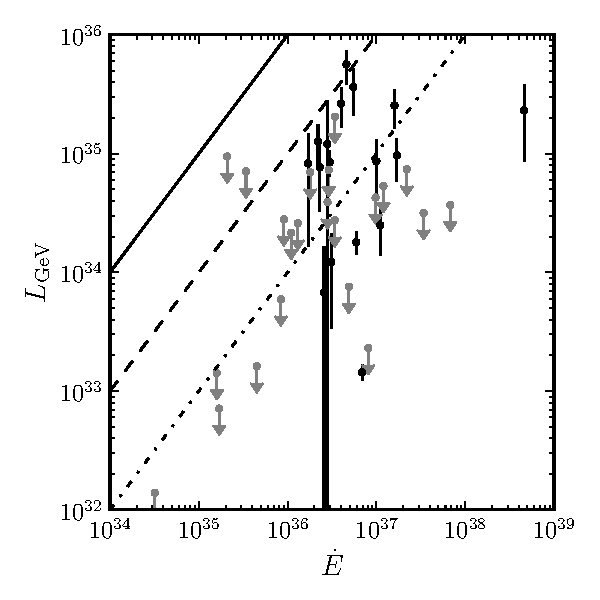
\includegraphics{chapters/population_study/figures/pwn_luminosity_vs_edot.pdf}
  \caption{The observed $\gamma$-ray luminosity compared to the observed
  spin-down luminosity for the \ac{PWN} candidates presented in
  \tabref{pwn_multiwavelenth_properties}.}
  \figlabel{pwn_luminosity_vs_edot}
\end{figure}

In \figref{pwn_luminosity_vs_edot}, we compare the observed luminosity at
\gev energies to the spin-down power of the observed pulsar.  This plot
shows that all \ac{LAT}-detected \acp{PWN} emmit a fraction $\lesssim
10\%$ of their spin-down energy goes into powering the $\gamma$-ray
emission from the pulsar wind.

\begin{figure}[htbp]
  \centering
  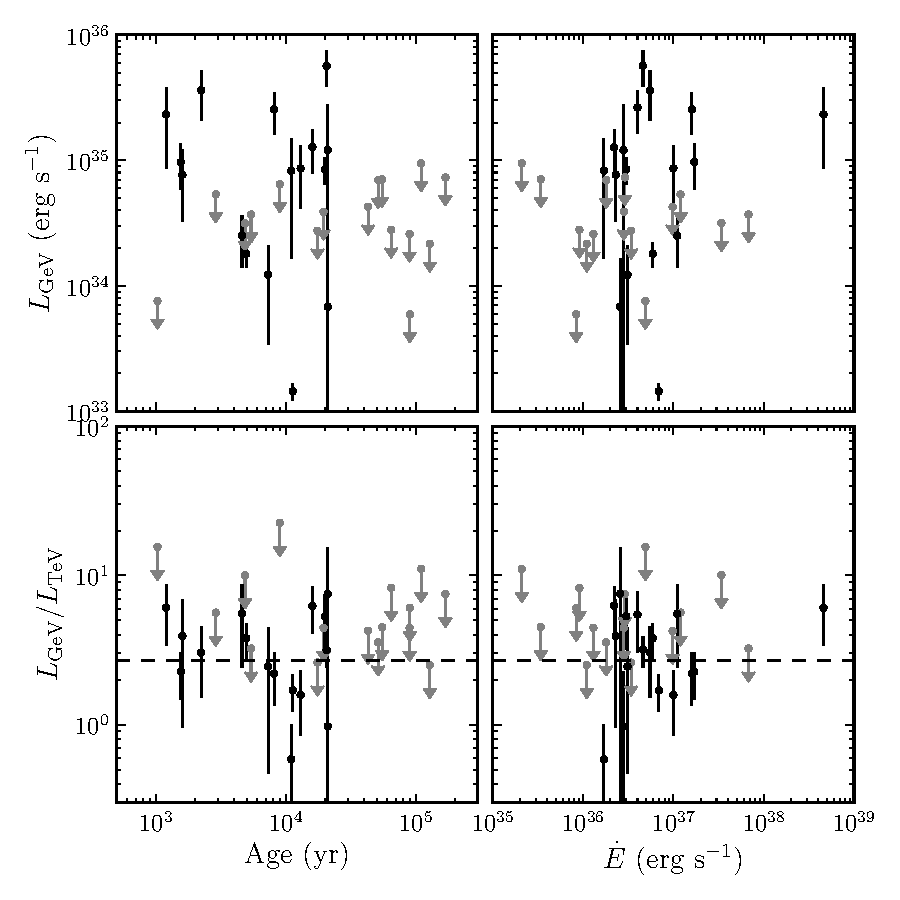
\includegraphics{chapters/population_study/figures/pwn_age_edot_vs_l_gev.pdf}
  \caption{The observed $\gamma$-ray luminosity and the
  \gev to \tev luminosity ratio as a
  function of the pulsar's age and spin-down energy
  for the \ac{PWN} candidates presented in
  \tabref{pwn_multiwavelenth_properties}.  The dotted line
  corresponds to the average luminosity ratio.  Because \hessj{1708}
  is classified as being a \PSRClass-type source in \chapref{tevcat},
  we consider it's observed $\gamma$-ray luminosity to be an upper limit
  on the \ac{PWN} emission.  \figlabel{pwn_age_edot_vs_l_gev.pdf}.}
\end{figure}

Next, in \figref{pwn_age_edot_vs_l_gev.pdf} we compare compare \gev
luminosity and \gev to \tev luminosity ratio as a function of age and
spin-down energy.  These plots shows that there is no correlation between
the \gev luminosity and the age and spin-down energy of the associate
pulsar.  In addition, we calculated and overlay the mean between the
\gev and \tev luminosity ($\MeanLuminosityRatio=2.7_{-1.4}^{+2.7}$).



\begin{figure}[htbp]
  \centering
  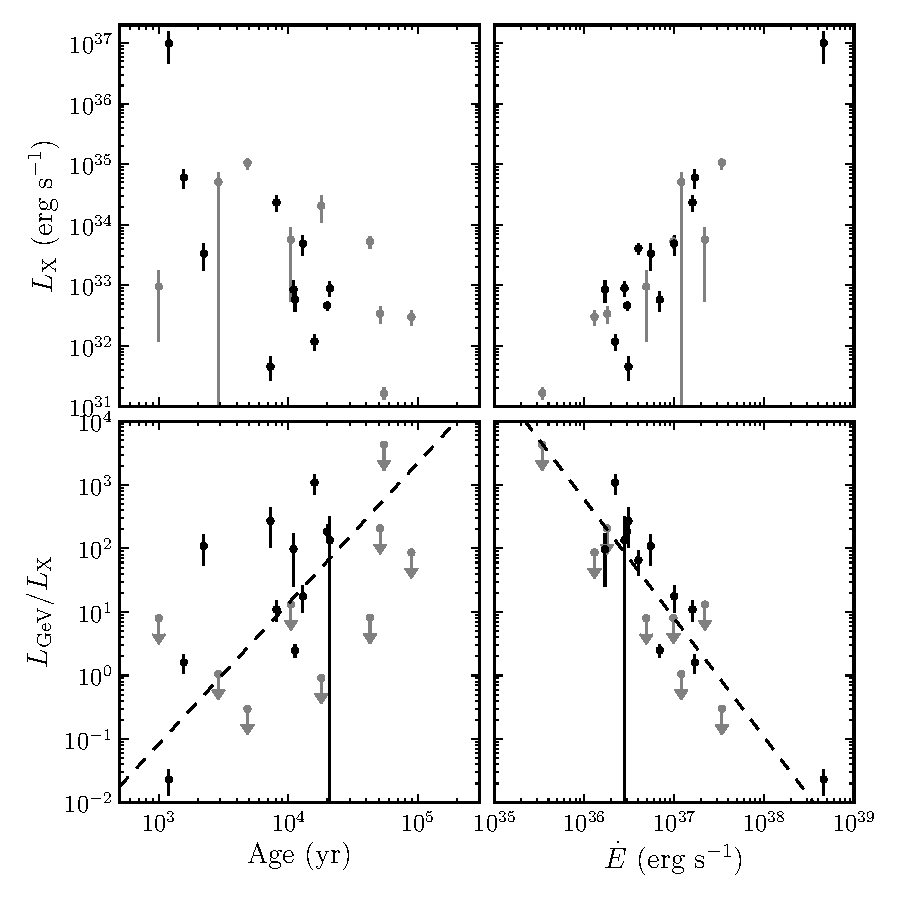
\includegraphics{chapters/population_study/figures/pwn_age_edot_vs_l_xray.pdf}
  \caption{The observed X-ray flux and \gev to \tev luminosity ratio as
  a function of the pulsar's age and spin-down energy for the \ac{PWN}
  candidates presented in \tabref{pwn_multiwavelenth_properties}.
  The dotted line corresponds to the scaling relationships from
  \cite{mattana_2009_evolution-gamma-} for the \tev to X-ray luminosity
  scaled by the average \gev to \tev luminosity (\MeanLuminosityRatio).
  We caution that \threecfiftyeight is not have a X-ray luminosity error.}
  \figlabel{pwn_age_edot_vs_l_xray}
\end{figure}

Finally, in \figref{pwn_age_edot_vs_l_xray} we compare the distribution
of the X-ray luminosity and the \gev to X-ray luminosity ratio as a
function of the pulsar's age and spin-down energy.  This plot shows
that the X-ray luminosity decreases with pulsar age and increases with
spin-down energy. Similarly, the \gev to X-ray luminosity increases
with age and decreases with energy.  These correlations are consistent
simple model predicted in \cite{mattana_2009_evolution-gamma-} (See
\secref{pwn_emission}) and also with the observed \ac{VHE} relationships
from the same paper.

